\chapter{Patternidentifikation}
Der nächste Schritt auf dem Weg zur lokalisierung der \QRCodes ist das identifizieren der \fps. Dafür wird die durch \OpenCV bereitgestellte \texttt{findContours} Methode verwendet. Sie basiert auf dem Algorithmus von Suzuki und wird eingesetzt um die Konturen aus dem Binärbild zu bestimmen.
\inputCPP[label={lst:findcontours}][][Aufruf der \texttt{findContours} Methode um die Konturen zu bestimmen.]{code/findContours.cpp}
Listing \ref{lst:findcontours} zeigt den Aufruf um alle Konturen des übergebenen Bildes zu erhalten.

\section{Vorgehensweise des Algorithmus von Suzuki} \label{suzuki}
Das Binärbild wird als durch iterriert. Für jeden Pixel $p_{i,j}$ werden folgende Bedingungen überprüft:
\begin{description}
	\item[outer border] Falls der Farbton des Vorgängers sich vom aktuell betrachteten Pixel unterscheidet. Beispielsweise für den Pixel $p_{i,j} = 1$ und $p_{i,j-1} = 0$ wäre $p_{i,j}$ ein Startpunkt einer \emph{outer border}. 
	\item[hole border] Falls der Farbton der Vorgänger sich in einem bestimmten Abstand gleich war, aber im aktuellen Pixel $p_{i,j}$ unterscheidet. Sei $x > 1$ ein beliebiger Abstand und es gelte $p_{i,j-x} =\ldots = p_{i,j-1}= 1$ und $p_{i,j} = 0$, dann ist $p_{i,j}$ ein Startpunkt einer \emph{hole border}.
\end{description}
Sind beide Bedingungen erfüllt, ist der Pixel $p_{i,j}$ ein Anfangspunkt einer neuen Kontur. Diese Kontur muss eindeutig identifizierbar sein daher wird sie mit einer \emph{KonturID} versehen. Der große Vorteil dieses Algorithmus ist die abgespeicherte Hierarchie der Konturen. Um dies zu gewährleisten, muss die \emph{parent}-Kontur für die neue Kontur gesetzt werden. Während des Scannens des Bildes wird immer die äußere Kontur zwischengespeichert, diese ist entweder die \emph{parent}-Kontur oder die Kontur die, die neue Kontur und die \emph{parent}-Kontur teilt. Wenn alle Werte gesetzt sind, wird die Kontur durch sukzessives Hinzunehmen von Pixeln entlang der Kante erzeugt. Das heißt es wird eine Kantenverfolgung durchgeführt. Nach jeder Kontur Erzeugung springt der Algorithmus zurück zum Raster Scan. Der Algorithmus terminiert bei Erreichen der rechten unteren Ecke.

Das Orginal Paper \cite{journals/cvgip/SuzukiA85} beschreibt ausfürlich das Vorgehen anhand Beispielen und Pseudocode.

\section{Filtern der Konturen}
Nachdem die Konturen bestimmt wurden, müssen die Konturen gefiltert werden da abhängig vom Bild können eine variable Anzahl an Konturen
erkannt werden. Beispielsweise werden bei der Ausführung der adaptiven Schwellwertoperation viele kleine Konturen erkannt. In folgenden Fällen werden Konturen ignoriert, da sie keine Aussagekraft besitzen.
\begin{enumerate}
	\item Die Kontur ist zu klein oder zu groß.
	\item Die Kontur besitzt kein \emph{parent}-Kontur.
	\item Konturen die Nachbarkonturen besitzen.
	\item Konturen die eine \emph{child}-Kontur besitzen.
\end{enumerate}
Für die äußeren Konturen also die \emph{parent}-Konturen müssen die Bedingungen 1.-3. natürlich auch gelten. Zusätzlich muss für die äußerste Kontur eine Trapezoide Form gelten. Um die letzte Bedingung zu überprüfen wird dazu die Form der Kontur mit \texttt{approxPolyDP} approximiert \todo{genauer erklären?}  und wenn diese aus genau vier Punkten besteht, wird es als Trapezoid anerkannt.

\section{Kanten approximieren}
Nachdem mehrere Kandidaten von \fps gefunden wurden, wird als nächstes die äußerste Kontur dieser Kandidaten verwendet um deren Kanten zu approximieren. Zuvor haben wir mit \OpenCV und Suzukis Algorithmus \ref{suzuki} alle Konturen mit \texttt{CV\_CHAIN\_APPROX\_NONE} im Bild lokalisiert, weswegen jede Kontur jetzt eine zusammenhängende Kette von Punkten darstellt. Für jeden Kandidat soll mit Hilfe dieser Punktmenge die Vier äußeren Kanten des \fps approximiert werden. Dazu teilen wir die Kontur in Vier Segmente auf und benutzen diese im späteren Verlauf um die Kanten zu approximieren.

Um die Schnittpunkte zu finden, an welchen die Kontur geteilt werden muss, werden die zuvor berechneten Vier Punkte, welche bereits genutzt wurden um festzustellen ob es sich bei der Kontur um ein Trapezoid handelt, verwendet. Diese liegen jedoch im Regelfall nicht exakt auf den Ecken der \fps und zusätzlich kann es durch schlechte Bildqualität zu abgerundeten oder leicht verschobenen Ecken im Originalbild kommen. Deswegen wird nachdem die Kontur zerteilt wurde, jeweils 10\% aller Punkte am Anfang und Ende jedes Segments verworfen, sodass ein Segment nur noch 80\% aller Punkte einer Kante beinhaltet. Diese Segmente werden dann genutzt um mit der \texttt{fitLine}-Methode die Kanten zu approximieren.

\begin{figure}[h]
\center
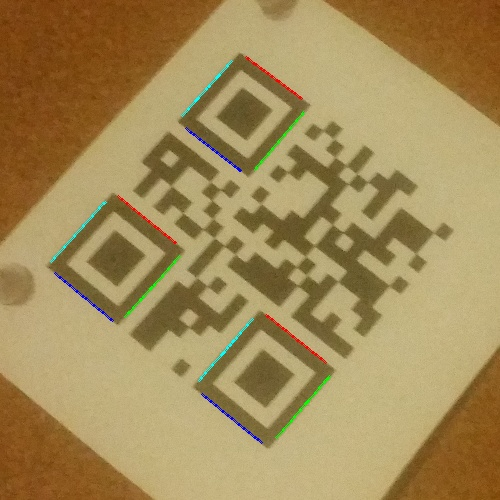
\includegraphics[scale=0.25]{images/qrcode-adler-wand_4___SEGMENTS___.jpg}
\hspace{5px}
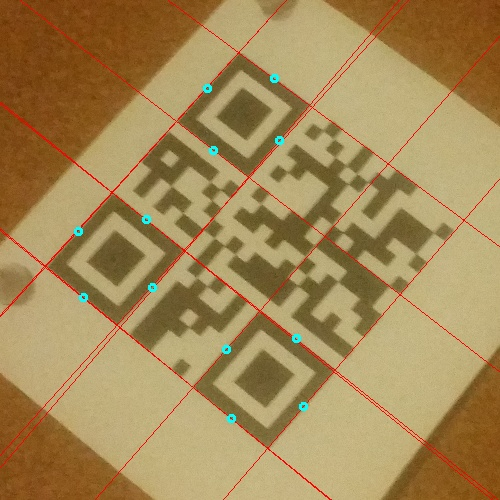
\includegraphics[scale=0.25]{images/qrcode-adler-wand_5___LINES___.jpg}
\caption{Links: Segmentierung der Konturen der \fps. Rechts: Approximation der Segmente durch Geraden.\label{fig:lines}}
\end{figure}

Die \texttt{fitLine}-Methode beruht auf dem Prinzip von \emph{M-Estimators} und verwendet als Minimierungsfunktion den in \OpenCV durch \texttt{CV\_DIST\_FAIR} definierten Ausdruck. Eine wichtige Eigenschaft dieser Methode ist, dass sie Geraden als einen Stützvektor und einen Richtungsvektor darstellt und der Stützvektor die Eigenschaft hat, sich innerhalb der konvexen Hülle aller Punkte zu befinden, welche zur Approximation verwendet wurden.
\\\\
Am Ende der Identifikation aller möglichen \fps erhält man somit folgende Informationen:
\begin{itemize}
	\item Mindestens drei \fp Kandidaten
	\item Eine Kontur pro \fp
	\item Vier Segmente pro \fp
	\item Vier Kantengeraden pro \fp
\end{itemize}